%%%%%%%%%%%%%%%%%%%%%%%%%%%%%%%%%%%%%%%%%
% Beamer Presentation
% LaTeX Template
% Version 2.0 (March 8, 2022)
%
% This template originates from:
% https://www.LaTeXTemplates.com
%
% Author:
% Vel (vel@latextemplates.com)
%
% License:
% CC BY-NC-SA 4.0 (https://creativecommons.org/licenses/by-nc-sa/4.0/)
%
%%%%%%%%%%%%%%%%%%%%%%%%%%%%%%%%%%%%%%%%%

%----------------------------------------------------------------------------------------
%	PACKAGES AND OTHER DOCUMENT CONFIGURATIONS
%----------------------------------------------------------------------------------------

\documentclass[
	11pt, % Set the default font size, options include: 8pt, 9pt, 10pt, 11pt, 12pt, 14pt, 17pt, 20pt
	%t, % Uncomment to vertically align all slide content to the top of the slide, rather than the default centered
	%aspectratio=169, % Uncomment to set the aspect ratio to a 16:9 ratio which matches the aspect ratio of 1080p and 4K screens and projectors
]{beamer}

\graphicspath{{Images/}{./}} % Specifies where to look for included images (trailing slash required)

\usepackage{booktabs} % Allows the use of \toprule, \midrule and \bottomrule for better rules in tables
\usepackage[russian]{babel}
% \usepackage[english,russian]{babel}
% \usepackage[dvipsnames]{xcolor}
% \usepackage{xcolor}

%----------------------------------------------------------------------------------------
%	SELECT LAYOUT THEME
%----------------------------------------------------------------------------------------

% Beamer comes with a number of default layout themes which change the colors and layouts of slides. Below is a list of all themes available, uncomment each in turn to see what they look like.

%\usetheme{default}
%\usetheme{AnnArbor}
%\usetheme{Antibes}
%\usetheme{Bergen}
%\usetheme{Berkeley}
%\usetheme{Berlin}
%\usetheme{Boadilla}
%\usetheme{CambridgeUS}
%\usetheme{Copenhagen}
%\usetheme{Darmstadt}
%\usetheme{Dresden}
%\usetheme{Frankfurt}
%\usetheme{Goettingen}
%\usetheme{Hannover}
%\usetheme{Ilmenau}
%\usetheme{JuanLesPins}
%\usetheme{Luebeck}
\usetheme{Madrid}
%\usetheme{Malmoe}
%\usetheme{Marburg}
%\usetheme{Montpellier}
%\usetheme{PaloAlto}
%\usetheme{Pittsburgh}
%\usetheme{Rochester}
%\usetheme{Singapore}
%\usetheme{Szeged}
%\usetheme{Warsaw}

%----------------------------------------------------------------------------------------
%	SELECT COLOR THEME
%----------------------------------------------------------------------------------------

% Beamer comes with a number of color themes that can be applied to any layout theme to change its colors. Uncomment each of these in turn to see how they change the colors of your selected layout theme.

%\usecolortheme{albatross}
%\usecolortheme{beaver}
%\usecolortheme{beetle}
%\usecolortheme{crane}
%\usecolortheme{dolphin}
%\usecolortheme{dove}
%\usecolortheme{fly}
%\usecolortheme{lily}
%\usecolortheme{monarca}
%\usecolortheme{seagull}
%\usecolortheme{seahorse}
%\usecolortheme{spruce}
%\usecolortheme{whale}
%\usecolortheme{wolverine}

%----------------------------------------------------------------------------------------
%	SELECT FONT THEME & FONTS
%----------------------------------------------------------------------------------------

% Beamer comes with several font themes to easily change the fonts used in various parts of the presentation. Review the comments beside each one to decide if you would like to use it. Note that additional options can be specified for several of these font themes, consult the beamer documentation for more information.

\usefonttheme{default} % Typeset using the default sans serif font
%\usefonttheme{serif} % Typeset using the default serif font (make sure a sans font isn't being set as the default font if you use this option!)
%\usefonttheme{structurebold} % Typeset important structure text (titles, headlines, footlines, sidebar, etc) in bold
%\usefonttheme{structureitalicserif} % Typeset important structure text (titles, headlines, footlines, sidebar, etc) in italic serif
%\usefonttheme{structuresmallcapsserif} % Typeset important structure text (titles, headlines, footlines, sidebar, etc) in small caps serif

%------------------------------------------------

%\usepackage{mathptmx} % Use the Times font for serif text
\usepackage{palatino} % Use the Palatino font for serif text

%\usepackage{helvet} % Use the Helvetica font for sans serif text
\usepackage[default]{opensans} % Use the Open Sans font for sans serif text
%\usepackage[default]{FiraSans} % Use the Fira Sans font for sans serif text
%\usepackage[default]{lato} % Use the Lato font for sans serif text
\usepackage{mathrsfs}
\usepackage{amsmath}
%----------------------------------------------------------------------------------------
%	SELECT INNER THEME
%----------------------------------------------------------------------------------------

% Inner themes change the styling of internal slide elements, for example: bullet points, blocks, bibliography entries, title pages, theorems, etc. Uncomment each theme in turn to see what changes it makes to your presentation.

%\useinnertheme{default}
\useinnertheme{circles}
%\useinnertheme{rectangles}
%\useinnertheme{rounded}
%\useinnertheme{inmargin}

%----------------------------------------------------------------------------------------
%	SELECT OUTER THEME
%----------------------------------------------------------------------------------------

% Outer themes change the overall layout of slides, such as: header and footer lines, sidebars and slide titles. Uncomment each theme in turn to see what changes it makes to your presentation.

%\useoutertheme{default}
%\useoutertheme{infolines}
%\useoutertheme{miniframes}
%\useoutertheme{smoothbars}
%\useoutertheme{sidebar}
%\useoutertheme{split}
%\useoutertheme{shadow}
%\useoutertheme{tree}
%\useoutertheme{smoothtree}

%\setbeamertemplate{footline} % Uncomment this line to remove the footer line in all slides
%\setbeamertemplate{footline}[page number] % Uncomment this line to replace the footer line in all slides with a simple slide count

%\setbeamertemplate{navigation symbols}{} % Uncomment this line to remove the navigation symbols from the bottom of all slides

%----------------------------------------------------------------------------------------
%	PRESENTATION INFORMATION
%----------------------------------------------------------------------------------------

\title[]{Пространственно-временная реконструкция временных рядов на основе тензорного разложения} % The short title in the optional parameter appears at the bottom of every slide, the full title in the main parameter is only on the title page

\author[Горишний Максим \and Надежда Алсаханова]{Горишний Максим \and Надежда Алсаханова} % Presenter name(s), the optional parameter can contain a shortened version to appear on the bottom of every slide, while the main parameter will appear on the title slide

\institute[]{МФТИ} % Your institution, the optional parameter can be used for the institution shorthand and will appear on the bottom of every slide after author names, while the required parameter is used on the title slide and can include your email address or additional information on separate lines

\date[\today]{\today} % Presentation date or conference/meeting name, the optional parameter can contain a shortened version to appear on the bottom of every slide, while the required parameter value is output to the title slide

%----------------------------------------------------------------------------------------

\begin{document}

%----------------------------------------------------------------------------------------
%	TITLE SLIDE
%----------------------------------------------------------------------------------------

\begin{frame}
	\titlepage % Output the title slide, automatically created using the text entered in the PRESENTATION INFORMATION block above
\end{frame}


%----------------------------------------------------------------------------------------
%	PRESENTATION BODY SLIDES
%----------------------------------------------------------------------------------------

\setbeamerfont{frametitle}{size=\normalsize}
%------------------------------------------------

\begin{frame}
	\frametitle{Цель исследования}

\begin{block}{Цель}
Сравнить Singular Spectrum Analysis (SSA) и его тензорную версию (TSSA) в пространственно-временном разложении и реконструкции временных рядов при сравнимой вычислительной затратности
\end{block}

\begin{block}{Идея}
TSSA за счет использования пространственной информации должен лучше справляться с задачей.
\end{block}

\begin{equation*}
L(\hat{x}) = MSE(x, \hat{x})
\end{equation*}

\end{frame}
%------------------------------------------------

\begin{frame}
    \frametitle{Постановка задачи}

\(x\) --- исходный временной ряд длины \(n\).

\(l\) --- длина окна для стадии эмбеддинга SSA.

\(m\) --- длина окна для стадии эмбеддинга TSSA.

\(\hat{x}\) --- реконструированный временной ряд.

\end{frame}

%------------------------------------------------

\begin{frame}
    \frametitle{Постановка задачи - SSA}
\small
\begin{gather*}
	X = [X_1, X_2, ..., X_{l}] = \mathcal{H} x = 
	 \begin{pmatrix}
		x_{1} & x_{2} & \dots & x_{l} \\
		x_{2} & x_{3} & \dots & x_{l + 1} \\
		\vdots & \vdots & \ddots & \vdots \\
		x_{l_{x}} & x_{l_x + 1} &  \dots & x_{l_x + l - 1}
	\end{pmatrix}, \notag \\
	l_x = n - l + 1;
\end{gather*}
\begin{gather*}
	X = \sum \limits_{i = 1}^{d} X_i = \sum \limits_{i = 1}^{d} \sqrt{\lambda_i} u_i v_i^T;
\end{gather*}
\begin{gather*}
	I = \{ I_1, I_2, \dots, I_q \}, \bigsqcup \limits_{i = 1}^{q} I = \{1, 2, \dots, d\} \notag \\
	\widehat{X} = \sum \limits_{i = 1}^{q} \widehat{X}_i = \sum \limits_{i = 1}^{q} \sum \limits_{j \in I_i} X_j;
\end{gather*}
\end{frame}

%------------------------------------------------

\begin{frame}
    \frametitle{Постановка задачи - TSSA}
\small
\begin{gather*}
	X = [X_1, X_2, ..., X_{k_x}] =
	 \begin{pmatrix}
		x_{1} & x_{2} & \dots & x_{m} \\
		x_{m+1} & x_{m+2} & \dots & x_{2m} \\
		\vdots & \vdots & \ddots & \vdots \\
		x_{k_{x}+1} & x_{k_x + 2} &  \dots & x_{k_x + m}
	\end{pmatrix} \text{, }\\
	k_x = \lfloor \frac{n}{m} \rfloor
\end{gather*}

\begin{gather*}
	\widehat{X} = PARAFAC(X) |_{first_k}
\end{gather*}

\end{frame}

%------------------------------------------------

\begin{frame} 
	\frametitle{Список литературы}
	
	\begin{thebibliography}{99} 
		\footnotesize
		
		\bibitem[Nina Golyandina, 2020]{p1}
			Nina Golyandina (2020)
			\newblock Particularities and commonalities of singular spectrum analysis as a method of time
			series analysis and signal processin

            \bibitem[Sanei Kouchaki, 2013]{p2}
			Sanei Kouchaki (2013)
			\newblock Tensor based singular spectrum analysis for nonstationary source separation

           \bibitem[aboba, 2015]{p3}
		   	DerkJan Dijk Samaneh Kouchaki, Saeid Sane (2015)
			\newblock Tensor based singular spectrum analysis for automatic scoring of sleep eeg

   		\bibitem[abiba, 2018]{p4}
		   	V.V. Strijov K.R. Usmanova. (2018)
			\newblock Models of detection relationship between time series in forecasting problems

	\end{thebibliography}
\end{frame}
%------------------------------------------------

\begin{frame}
    \frametitle{Данные}
\scriptsize

Ситнтетичиские квази-периодические ряды длины \(n = 1000\)

Продажи топлива в день на протяжении года \(n = 365\)

Потребление электричества в час на протяжении года \(n = 8760\)

\begin{figure}
	\centering
	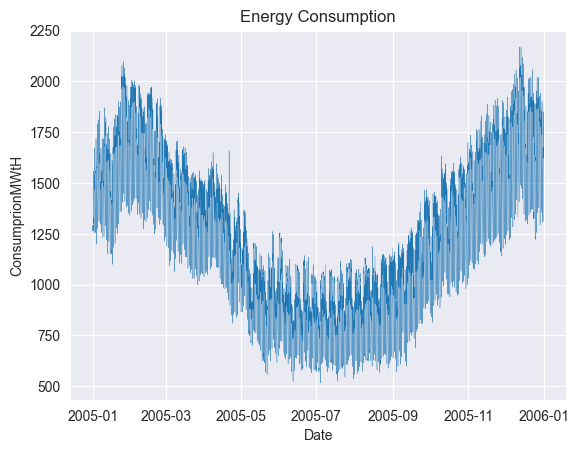
\includegraphics[width=0.6\textwidth]{images/energy.png}
	\label{fig:test}
\end{figure}

\end{frame}
%------------------------------------------------

\begin{frame}
    \frametitle{Решение}

Для SSA --- перебор размера окна \(l\) и выбор первых компонент \(k\) по сетке с шагом 1.

Для TSSA --- перебор размера окна \(m\), ганкелизация с размером \(l\) и выбор первых компонент \(k\) по сетке с шагом 1.

\end{frame}
%------------------------------------------------

\begin{frame}
	\frametitle{Результаты}

\begin{figure}
	\centering
	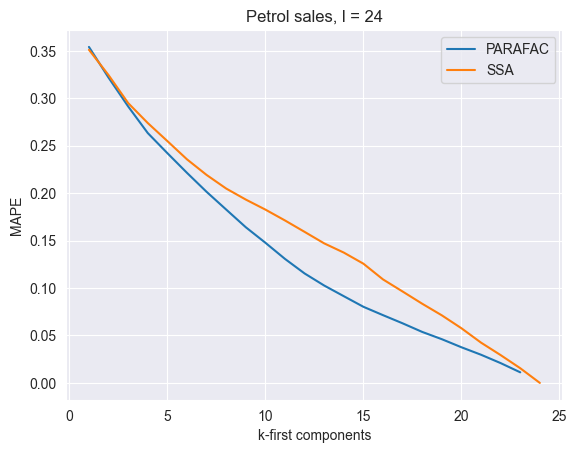
\includegraphics[width=0.5\textwidth]{images/result_good.png}%
	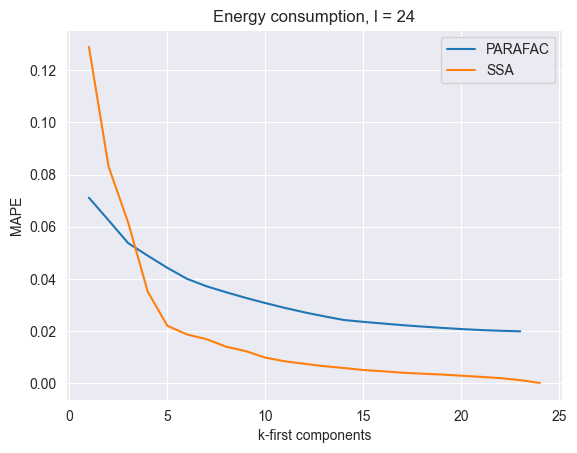
\includegraphics[width=0.5\textwidth]{images/result_bad.png}
	\label{fig:result}
\end{figure}

На малых \(k\) TSSA показывает лучшие результаты, чем SSA. На больших \(k\) соотношение их точности зависит от данных и гиперпараметров.

\end{frame}

%------------------------------------------------

\begin{frame}
	\frametitle{Заключение}

\begin{itemize}
	\item SSA практически не требует подбора гиперпараметров
    \item TSSA более устойчив и точен, но требует более тонкого подбора гиперпараметров
    \item В большинстве случаев TSSA работает медленнее SSA
    \item Алгоритмы не заменяют, а дополняют друг друга
\end{itemize}

\end{frame}

%------------------------------------------------------------------------------
%	CLOSING SLIDE
%------------------------------------------------------------------------------

% \begin{frame}[plain] % The optional argument 'plain' hides the headline and footline
% 	\begin{center}	
% 		\bigskip\bigskip % Vertical whitespace
% 		{\LARGE Спасибо за внимание!}
% 	\end{center}
% \end{frame}

%----------------------------------------------------------------------------------------

\end{document} 